\subsection{Display > Camera settings}
\label{subsection:cameraSettings}

Ce dialogue, associ� � la vue 3D active, permet de modifier l'orientation et la cam�ra (via 3 angles : $\Theta$, $\Phi$ et $\Psi$) ainsi que son centre de rotation (pivot) et son ouverture angulaire (f.o.v. pour "<field of view"> - applicable uniquement en vision perspective).\\

Il est aussi possible de :
\begin{itemize}
\item stocker l'orientation courante (ic�ne "<caddie">)
\item r�tablir l'orientation pr�c�demment stock�e (ic�ne suivante)
\item et enfin appliquer une des 6 orientations pr�-d�finies (haut, bas, gauche, droite, devant,
derri�re) relativement � la position stock�e (6 derni�res ic�nes)\\
\end{itemize}

\begin{center}
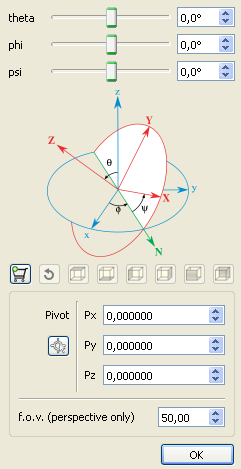
\includegraphics[width=0.3\textwidth]{images/Partie3_Fonctions/CameraParameters}
\par\end{center}
